%%%%%%%%%%%%%%%
\task{Шутка}
\begin{itemize}
\itA Стул с пятнадцатью ножками упал с лестницы из пяти ступенек и сломал одну ножку. Потом он упал с лестницы из десяти ступенек и сломал три ножки. Сколько ножек он сломает, упав с лестницы из 20 ступенек?

\itB За книгу заплатили 200 рублей, и осталось заплатить втрое больше, чем осталось бы заплатить, если бы заплатили половину заплаченного и ещё столько, сколько осталось заплатить. Сколько стоит книга?

\itC Известно, что Магеллан израсходовал на день больше, чем рассчитывал, при движении с востока на запад. В свою очередь, герои книги «Вокруг света за 80 дней» экономили время при движении с запада на восток. Но можно ли изменить скорость времени, просто начав бегать вокруг Северного полюса?
\end{itemize}
%%%%%%%%%%%%%%%

%%%%%%%%%%%%%%%
\task{Числа и суммы}
\begin{itemize}
\itA Может ли число быть меньше количества цифр в нём? Может ли число быть меньше собственной суммы цифр?

\itB Как по натуральному числу $n$ найти число, не превосходящее его, с наибольшей суммой цифр?

\itC Петя сложил все числа от 1 до $m \cdot n$, а Вася сложил все числа от 1 до $m$, от 1 до $n$ и посчитал произведение этих двух сумм. У кого в итоге получилось большее число?
\end{itemize}
%%%%%%%%%%%%%%%

%%%%%%%%%%%%%%%
\task{Деление и остатки}
\begin{itemize}
\itA В преддверии олимпиады «Математика НОН-СТОП» Настя решила поупражняться в делении чисел. Она придумала некоторое число, и у неё получилось, что это число делится на 564. Ещё она выяснила, что 2016 делится на это число. Права ли Настя?

\itB Всё те же подруги теперь тренируются считать остатки от деления числа на число. Первая берёт число $a$, считает его остаток от деления на число $b$, а затем считает остаток от деления этого остатка на число $c$. Вторая утверждает, что процесс можно ускорить, сразу считая остаток от деления $a$ на $c$, без потери правильности ответа. Права ли она? Если да, докажите это, если нет — приведите контрпример.

\itC Даны два числа $b$ и $c$. Доказать, что для любого $a$ выполнено $(a \bmod b) \bmod c = a \bmod c$ тогда и только тогда, когда $b$ делится на $c$.
\end{itemize}
%%%%%%%%%%%%%%%

%%%%%%%%%%%%%%%
\task{Спички и пионеры}
\begin{itemize}
\itA Пионер Петя выкладывает цифры из спичек так, как это делается на экране стандартного калькулятора. Какое наибольшее число он может сложить из 15 спичек?

\itB Могло ли случиться так, что в петином отряде из 20 пионеров имена у всех начинаются с разных букв?

\itC Тем временем пионер Вася хочет научиться выкладывать цифры наименьшим числом спичек. Помогите ему в этом: найдите наименьшее число $k$ такое, что любая цифра может быть выложена из $k$ спичек. 
\end{itemize}

\begin{center}
  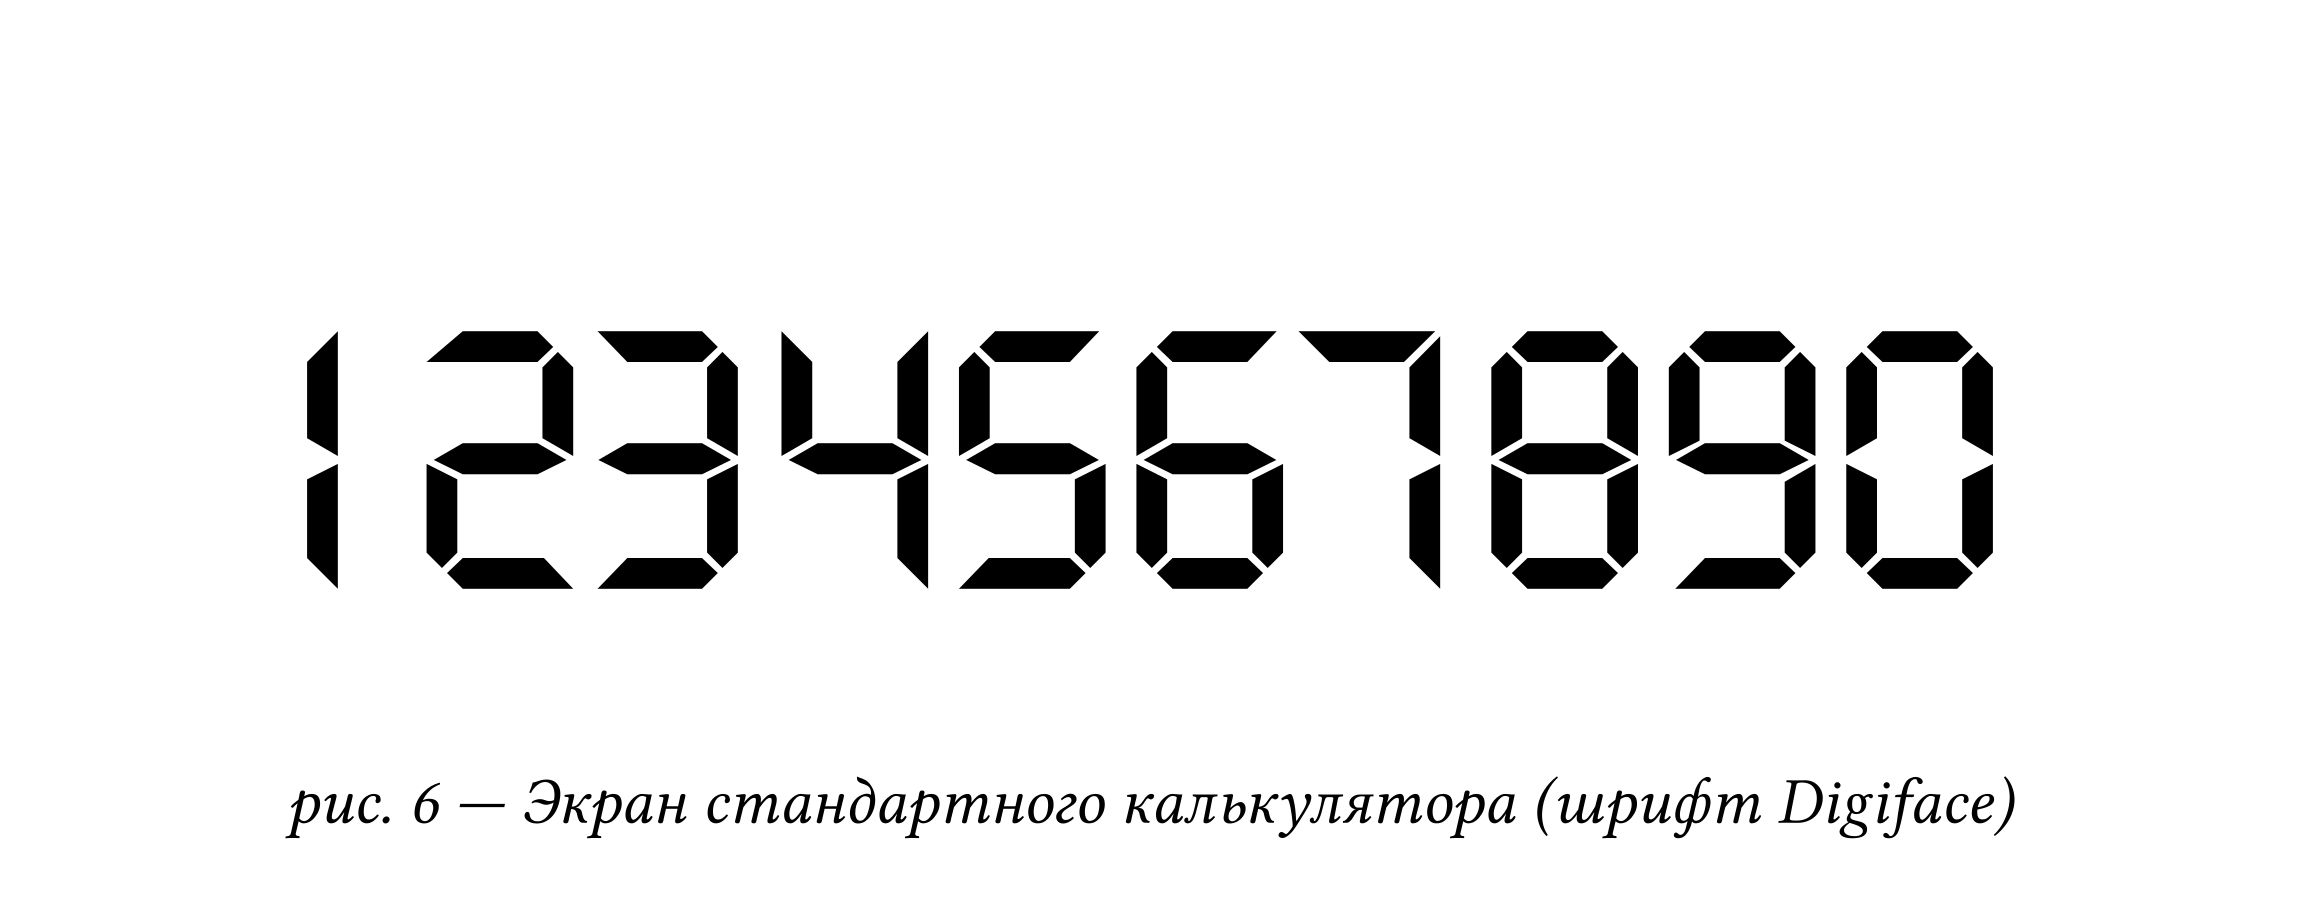
\includegraphics[width=6cm]{stats/2016/Figures/Digiface.png}
\end{center}
%%%%%%%%%%%%%%%

%%%%%%%%%%%%%%%
\task{Плохая компания}
\begin{itemize}
\itA В компании из 10 человек среди любых пятерых — не более трёх девочек. Какое наибольшее число девочек может быть в компании?

\itB В стране 140'000'000 людей. Министру здравоохранения донесли, что среди 35 миллионов и одного человека всегда есть хоть один носитель опасного вируса Нойвис-припг. Министр прикинул в голове: это ведь получается, что ничтожно малая доля населения страны является носителем вируса! Прав ли он?

\itC Дана компания из $N$ человек. Известно, что из $p$ людей по крайней мере $q$ --- девочки, а из $s$ девочек по крайней мере $t$ --- блондинки. Какое наименьшее количество блондинок может быть в этой компании?
\end{itemize}
%%%%%%%%%%%%%%%

%%%%%%%%%%%%%%%
\task{Эти необычные механизмы}
\begin{itemize}
\itA Федя собрал систему из шестерёнок, как на рисунке 1. Будут ли шестерёнки вращаться?

\itB В японских шахматах сёги есть фигура Золото, которая бьёт шесть клеток вокруг себя (закрашены серым на рисунке 2). Можно ли расставить на поле $9 \times 9$ несколько таких фигур, чтобы каждая клетка поля билась ровно одним Золотом?

\itC Конструкция самосвала такова, что он может ехать, потеряв до четырёх колёс. Правда, его максимальная скорость, равная 60 км/ч, уменьшается на 6 км/ч с каждым потерянным колесом. Раз в 12 км на шоссе встречаются шиномонтажи, где разговор с работником занимает 10 минут, а установка каждого колеса — по 3 минуты. Сразу же после выезда с / проезда мимо очередного шиномонтажа у самосвала отваливается одно колесо. Сколько колёс выгоднее всего терять водителю между двумя заездами на шиномонтаж, если он хочет в среднем ехать как можно быстрее?
\end{itemize}

\begin{center}
  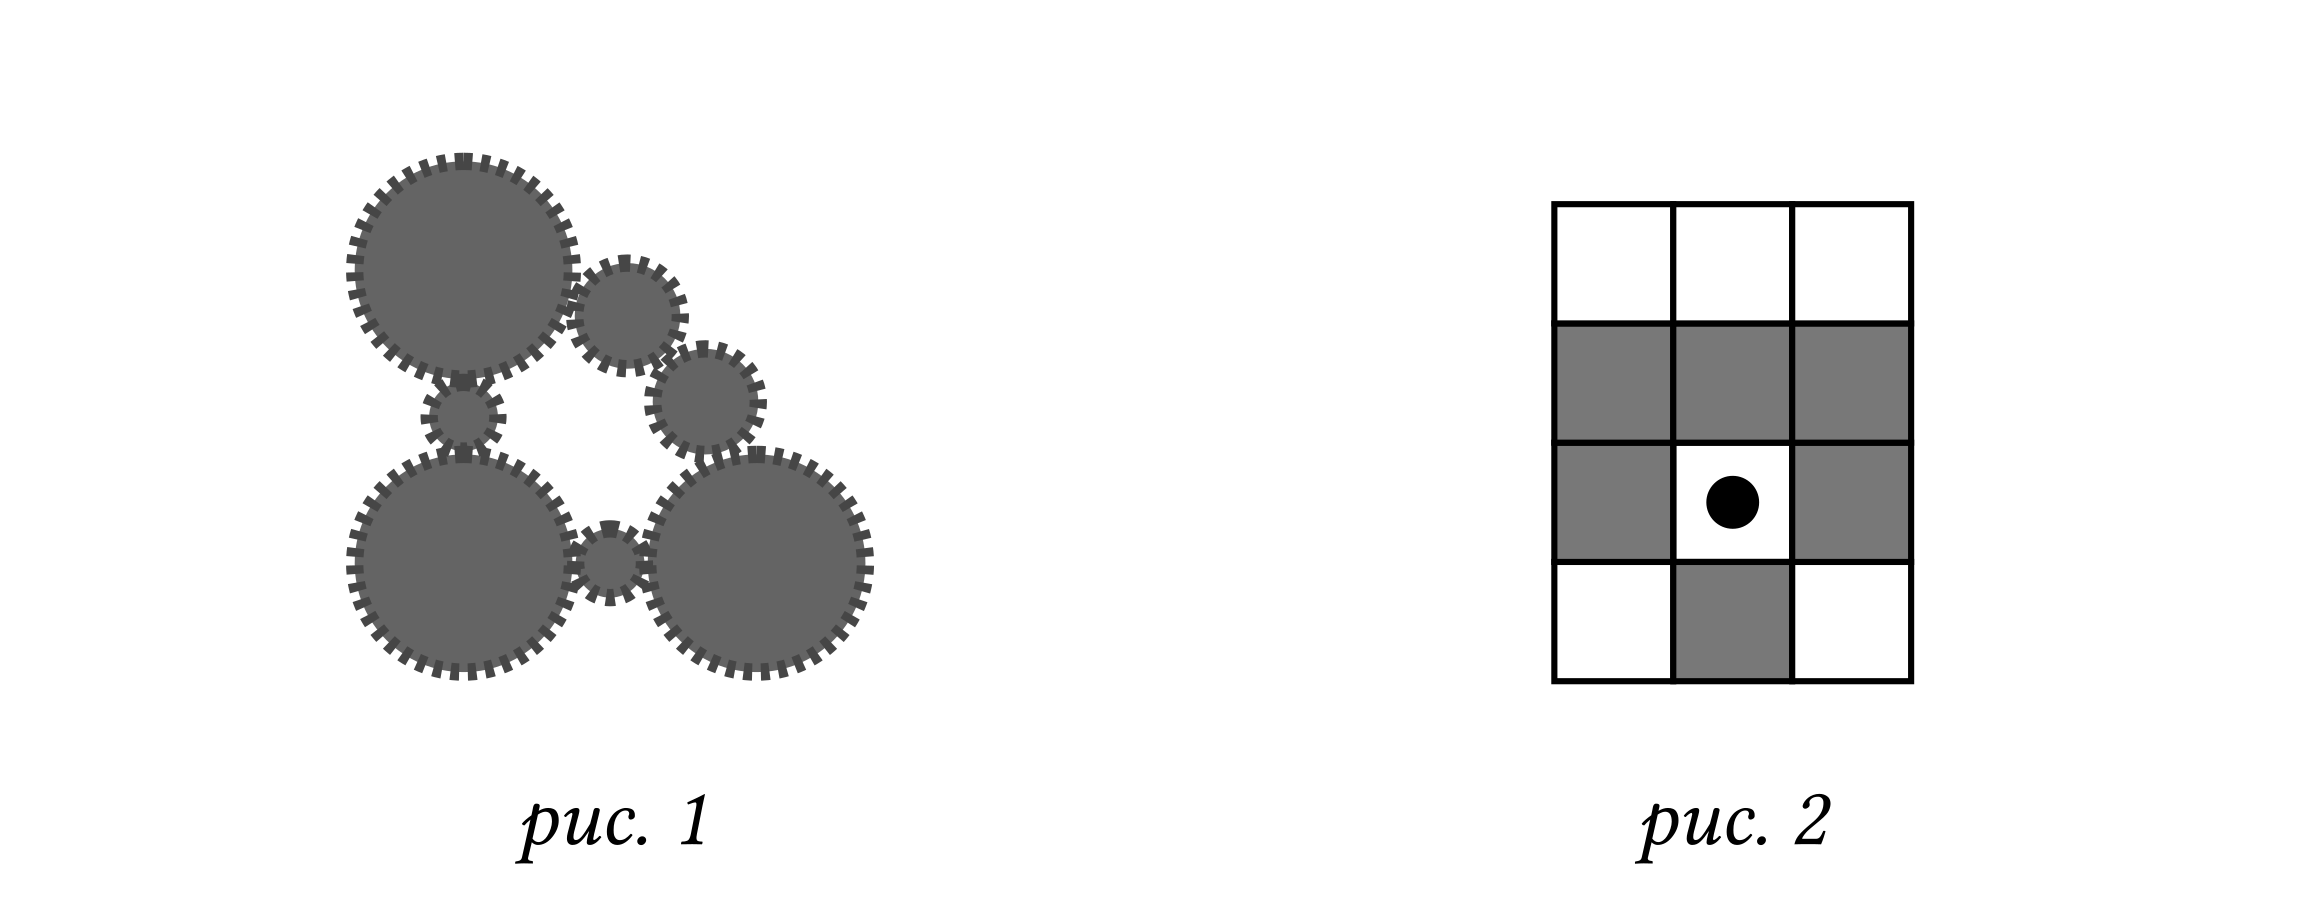
\includegraphics[width=8cm]{stats/2016/Figures/Gears_and_Arrow.png}
\end{center}
%%%%%%%%%%%%%%%